\documentclass{article}

\usepackage{microtype}
\usepackage{graphicx}
\usepackage{subfigure}
\usepackage{booktabs} % for professional tables
\usepackage{xr-hyper} % for referencing appendix

%%%%%%%%%%%%%%%%%%%%%%%%%%%%%%%%%%%%%%%%%%%%%%%%%%%%%%%%%%%%
%%%%%% Additional code for cross referencing appendix %%%%%%
%%%%%%%%%%%%%%%%%%%%%%%%%%%%%%%%%%%%%%%%%%%%%%%%%%%%%%%%%%%%
\makeatletter
\newcommand*{\addFileDependency}[1]{% argument=file name and extension
  \typeout{(#1)}
  \@addtofilelist{#1}
  \IfFileExists{#1}{}{\typeout{No file #1.}}
}
\makeatother
 
\newcommand*{\myexternaldocument}[1]{%
    \externaldocument{#1}%
    \addFileDependency{#1.tex}%
    \addFileDependency{#1.aux}%
}
\myexternaldocument{appendix}
%%%%%%%%%%%%%%%%%%%%%%%%%%%%%%%%%%%%%%%%%%%%%%%%%%%%%%%%%%%%
%%%%%%%%%%%%%%%%%%%%%%%%%%%%%%%%%%%%%%%%%%%%%%%%%%%%%%%%%%%%

\usepackage{hyperref}
\newcommand{\theHalgorithm}{\arabic{algorithm}}

\usepackage{icml2020}

\usepackage[utf8]{inputenc}
\usepackage{amsmath, mathrsfs, mathtools, amsfonts, amsthm}
\usepackage{color}
\allowdisplaybreaks

\newtheorem{proposition}{Proposition}

\icmltitlerunning{Interpretable Off-Policy Evaluation by Highlighting Influential Transitions}

\begin{document}

\twocolumn[
\icmltitle{Interpretable Off-Policy Evaluation in Reinforcement Learning \texorpdfstring{\\}{} by Highlighting Influential Transitions}

\icmlkeywords{off-policy evaluation, interpretability}

\vskip 0.3in
]

\begin{abstract}
    Off-policy evaluation in reinforcement learning offers the chance of using observational data to improve future outcomes in domains such as healthcare and education, but safe deployment in high stakes settings requires ways of assessing its validity. Traditional measures such as confidence intervals may be insufficient due to noise, limited data and confounding. In this paper we develop a method that could serve as a hybrid human-AI system, to enable human experts to analyze the validity of policy evaluation estimates. This is accomplished by highlighting observations in the data whose removal will have a large effect on the OPE estimate, and formulating a set of rules for choosing which ones to present to domain experts for validation. We develop methods to compute exactly the influence functions for fitted Q-evaluation with two different function classes: kernel-based and linear least squares. Experiments on medical simulations and real-world intensive care unit data demonstrate that our method can be used to identify limitations in the evaluation process and make evaluation more robust.
\end{abstract}

\section{Introduction}

Within reinforcement learning (RL), off-policy evaluation (OPE) is the task of estimating the value of a given evaluation policy, using data collected by interaction with the environment under a different behavior policy \citep{sutton2018reinforcement, precup2000eligibility}. OPE is particularly valuable when interaction and experimentation with the environment is expensive, risky, or unethical---for example, in healthcare or with self-driving cars. However, despite recent interest and progress, state-of-the-art OPE methods still often fail to differentiate between obviously good and obviously bad policies, e.g. in healthcare \citep{gottesman2018evaluating}.

Most of the OPE literature focuses on sub-problems such as improving asymptotic sample efficiency or bounding the error on OPE estimators for the value of a policy. However, while these bounds are theoretically sound, they are often too conservative to be useful in practice (though see e.g.~\citet{thomas2019} for an exception). This is not surprising, as there is a theoretical limit to the statistical information contained in a given dataset, no matter which estimation technique is used. Furthermore, many of the common assumptions underlying these theoretical guarantees are usually not met in practice: observational healthcare data, for example, often contains many unobserved confounders \citep{gottesman2019guidelines}.

Given the limitations of OPE, we argue that in high stakes scenarios domain experts should be integrated into the evaluation process in order to provide useful actionable results. For example, senior clinicians may be able to provide insights that reduce our uncertainty of our value estimates. In this light, the explicit integration of expert knowledge into the OPE pipeline is a natural way for researchers to receive feedback and continually update their policies until one can make a responsible decision about whether to pursue gathering prospective data.

The question is then what information can humans provide that might help assess and potentially improve our confidence in an OPE estimate? In this work, we consider how human input could improve our confidence in the recently proposed OPE estimator, fitted Q-evaluation (FQE) \cite{le2019batch}.  We develop an efficient approach to identify the most influential transitions in the batch of observational data, that is, transitions whose removal would have large effects on the OPE estimate. By presenting these influential transitions to a domain expert and verifying that they are indeed representative of the data, we can increase our confidence that our estimated evaluation policy value is not dependent on outliers, confounded observations, or measurement errors. The main contributions of this work are:

\begin{itemize}
    \item \emph{Conceptual}: We develop a framework for using influence functions to interpret OPE, and discuss the types of questions which can be shared with domain experts to use their expertise in debugging OPE.
    \item \emph{Technical}:  We develop computationally efficient algorithms to compute the exact influence functions for two broad function classes in FQE: kernel-based functions and linear functions.
    \item \emph{Empirical}: We demonstrate the potential benefits of influence analysis for interpreting OPE on a cancer simulator, and present results of analysis together with practicing clinicians of OPE for management of acute hypotension from a real intensive care unit (ICU) dataset.
\end{itemize}

\section{Related work}

The OPE problem in RL has been studied extensively.  Works fall into three main categories: importance sampling (IS) (e.g. \citet{precup2000eligibility, jiang2015doubly}), model-based (often referred to as the direct method) (e.g. \citet{hanna2017bootstrapping, gottesman2019combining}), and value-based (e.g. \citet{le2019batch}). Some of these works provide bounds on the estimation errors (e.g. \citet{thomas2015high, dann2018policy}). We emphasize, however, that for most real-world applications these bounds are either too conservative to be useful or rely on assumptions which are usually violated.

While there has been considerable recent progress in interpretable machine learning and machine learning with humans in the loop (e.g. \citet{tamuz2011adaptively, lage2018human}), to our knowledge, there has been little work that considers human interaction in the context of OPE. \citet{oberst2019counterfactual} proposed framing the OPE problem as a structural causal model, which enabled them to identify trajectories where the predicted counterfactual trajectories under an evaluation policy differs substantially from the observed data collected under the behavior policy. However, that work does not give guidance on what part of the trajectory might require closer scrutiny, nor can it use human input for additional refinement. 

Finally, the notion of influence that we use throughout this work has a long history in statistics as a technique for evaluating the robustness of estimators \citep{cook1980characterizations}.  Recently, an approximate version of influence for complex black-box models was presented in \citet{koh2017understanding}, and they demonstrated how influence functions can make machine learning methods more interpretable. In the context of optimal control and RL, influence functions were first introduced by \citet{munos2002variable} to aid in online optimization of policies. However, their definition of influence as a change in the value function caused by perturbations of the reward at a specific state is quite different from ours. 

\section{Background}

\subsection{Notation}

A Markov Decision Process (MDP) is a tuple $\langle \mathcal{X}, \mathcal{A}, P_T, P_R, P_0, \gamma \rangle$, where $\mathcal{X}$, $\mathcal{A}$ and $\gamma$ are the state space, action space, and the discount factor, respectively. The next state transition and reward distributions are given by $P_T(\cdot | x, a)$ and $P_R(\cdot | x, a)$ respectively, and $P_0(x)$ is the initial state distribution. The state and action spaces could be either discrete or continuous, and the transition and reward functions may be either stochastic or deterministic. 

A dataset is composed of a set of $N$ observed transitions $\mathcal{D} =  \{ (x^{(n)}, a^{(n)} ,r^{(n)} ,x'^{(n)}) \}_{n=1}^N$, and we use $\tau^{(n)}$ to denote a single transition. The subset $\mathcal{D}_0 \subseteq \mathcal{D}$ denotes initial transitions from which $P_0$ can be estimated. Note that although we treat all data points as observed transitions, in most practical applications data is collected in the form of trajectories rather than individual transitions.

A policy is a function $\pi : (\mathcal{X}, \mathcal{A}) \rightarrow \left[0, 1 \right]$ that gives the probability of taking each action at a given state $(\sum_{a \in \mathcal{A}} \pi(a|x) = 1)$.  The value of a policy is the expected return collected by following the policy, $v^\pi \coloneqq \mathrm{E} [ g_T | a_t \sim \pi]$, where actions are chosen according to $\pi$, expectations are taken with respect to the MDP, and $g_T \coloneqq \sum_{t=0}^T \gamma^t r_t$ denotes the total return, or sum of discounted rewards. The state-action value function $q^{\pi}(x, a)$ is the expected return for taking action $a$ at state $x$, and afterwards following $\pi$ in selecting future actions. The goal of off-policy evaluation is to estimate the value of an \emph{evaluation} policy, $\pi_e$, using data collected using a different \emph{behavior} policy $\pi_b$. In this work, we are only interested in estimating $v^{\pi_e}$ and $q^{\pi_e}$, and will therefore drop the superscript for brevity. We will also limit ourselves to deterministic evaluation policies.

For the purpose of kernel-based value function approximation, we define a distance metric, $d((x^{(i)}, a^{(i)}),(x^{(j)}, a^{(j)}))$ over $\mathcal{X} \times \mathcal{A}$. In this work, for discrete action spaces, we will assume $d((x^{(i)}, a^{(i)}),(x^{(j)}, a^{(j)})) = \infty$ when $a^{(i)} \neq a^{(j)}$, but this is not required for any of the derivations.

\subsection{Fitted Q-Evaluation}

Fitted Q-Evaluation \citep{le2019batch} can be thought of as dynamic programming on an observational dataset to compute the value of a given evaluation policy. It is similar to the more well-known fitted Q-iteration method (FQI) \citep{ernst2005tree}, except it is performed offline on observational data, and the target is used for evaluation of a given policy rather than for optimization. FQE performs a sequence of supervised learning steps where the inputs are state-action pairs, and the targets at each iteration are given by $y_i(x, a) = r + \gamma \hat{q}_{i-1}(x', \pi_e(x'))$, where $\hat{q}_{i-1}(x, a)$ is the estimator (from a function class $\mathcal{F}$) that best estimates $y_{i-1}(x, a)$. For more information, see \citet{le2019batch}.

\section{OPE diagnostics using influence functions}

\subsection{Definition of the influence}

We aim to make OPE interpretable and easy to debug by identifying transitions in the data which are highly influential on the estimated policy value. We define the \emph{total influence} of transition $\tau^{(j)}$ as the change in the value estimate if $\tau^{(j)}$ was removed:
\begin{equation}
    I_j \equiv \hat{v}_{-j} - \hat{v},
\end{equation}
where $\hat{v}_{-j}$ is the value estimate using the same dataset after removal of $\tau^{(j)}$. In general, for any function of the data $f(\mathcal{D})$ we will use $f(\mathcal{D}_{-j}) \equiv f_{-j}$ to denote the value of $f$ computed for the dataset after removal of $\tau^{(j)}$.

Another quantity of interest is the change in the estimated value of $q(x^{(i)}, a^{(i)})$ as a result of removing $\tau^{(j)}$, which we call the \emph{individual influence}:
\begin{equation}
    I_{i, j} \equiv \hat{q}_{-j}(x^{(i)}, a^{(i)}) - \hat{q}(x^{(i)}, a^{(i)}).
\end{equation}
The total influence of $\tau^{(j)}$ can be computed by averaging its individual influences over the set $\mathcal{D}^*_0$ of all initial state-action transitions in which $a=\pi_e(x)$: 
\begin{equation}
    I_j = \frac{1}{|\mathcal{D}^*_0|} \sum_{i \in \mathcal{D}^*_0} I_{i, j}.
\end{equation}
As we are interested in the robustness of our evaluation, we can normalize the absolute value of the influence of $\tau^{(j)}$ by the estimated value of the policy to provide a more intuitive notion of overall importance:
\begin{equation}
    \tilde{I}_j \equiv \frac{|I_j|}{|\hat{v}|}.
\end{equation}

\subsection{Diagnosing OPE estimation}

With the above definitions of influence functions, we now formulate and discuss guidelines for diagnosing the OPE process for potential problems. 

\paragraph{No influential transitions: OPE appears reliable.}  
As a first diagnostic, we check that none of the transitions influence the OPE estimate by more than a specified influence threshold $\tilde{I}_C$, i.e. for all $j$ we have $\tilde{I}_j \leq \tilde{I}_C$. In such a case we would output that, to the extent that low influences suggests the OPE is stable, the evaluation appears reliable. That said, we emphasize that our proposed method for evaluating OPE methods is not exhaustive, and there could be many other ways in which OPE could fail.

\paragraph{Influential transitions: a human can help.}
When there are several influential transitions in the data (defined as transitions whose influence is larger than $\tilde{I}_C$), we present them to domain experts to determine whether they are representative, that is, taking action $a$ in state $x$ is likely to result in transition to $x'$.  If the domain experts can validate all influential transitions, we can still have some confidence in the validity of the OPE. If any influential transitions are flagged as unrepresentative or artefacts, we have several options: (1) Declare the OPE as unreliable; (2) Remove the suspect influential transitions from the data and recompute the OPE; (3) Caveat the OPE results as valid only for a subset of initial states that do not rely on that problematic transition.

In situations where there is a large number of influential transitions, manual review by experts may be infeasible. As such, it is necessary to present as few transitions as possible while still presenting enough to ensure that any potential artefacts in the data and/or the OPE process are accounted for. In practice, we find it is common to observe a sequence of influential transitions where removing any single transition has the same effect as removing the entire sequence. An example of this is shown schematically in Figure \ref{fig:influential_sequence}. An entire sequence marked in blue and red leads to a region of high reward, and so all transitions in that sequence will have high influence. The whole influential sequence appears very different from the rest of the data, and a domain expert might flag it as an outlier to be removed. However, we can present the expert with only the red transition and capture the influence of the blue transitions as well, reducing the number of suspect examples to be manually reviewed.

\paragraph{Influential transitions: policy is unevaluatable.}  When an influential transition, $\tau^{(j)}$, has no nearest neighbors to $(x'^{(j)}, \pi_e(x'^{(j)}))$, we can determine that the evaluation policy cannot be evaluated, even without review by a domain expert. This claim is a result of the fact that such a situation represents reliance of the OPE on transitions for which there is no overlap between the actions observed in the data and the evaluation policy. However, while the evaluation policy is not evaluatable, the influential ``dead-end'' transitions may still inform experts of what data is required for evaluation to be feasible.

It should be noted that the applicability of the diagnostics methods discussed above may change depending on whether the FQE function class is parametric or nonparametric. All function classes lend themselves to highlighting of highly influential transitions. However, the notion of stringing together sequences of neighbors, or looking for red flags in the form of influential transitions with no neighbors to their $(x', \pi_e(x'))$ state action pairs only makes sense for nonparametric models. In the case of parametric models, the notion of neighbors is less important as the influence of removing a transition manifests as a change to the learned parameters which affects the value estimates for the entire domain simultaneously. In contrast, for nonparametric methods, removing a transition locally changes the value of neighboring transitions and propagates through the entire domain through the sequential nature of the environment. While we derive efficient ways to compute the influence for both parametric and nonparametric function classes, in the empirical section of this paper we present results for nonparametric kernel-based estimators to demonstrate all diagnostics.

\begin{figure}[t]
\centering
\includegraphics[width=0.3\textwidth]{influential_sequence.pdf}
\caption{\textbf{Schematic of an influential sequence.} All transitions in the sequence leading to a high reward have high influence, but flagging just the red transition for inspection will capture the influence of the blue ones as well.}\label{fig:influential_sequence}
\end{figure}

\section{Efficient computation of influence functions}
\label{sec:computation_of_influence}

A key technical challenge in performing the proposed influence analysis in OPE is computing the influences efficiently. The brute-force approach of removing a transition and recomputing the OPE estimate is clearly infeasible for all but tiny problems, as it requires refitting $N$ models. The computation of influences in RL is also significantly more challenging than in static one-step prediction tasks, as a change in the value of one state has a ripple effect on all other states that are possible to reach from it. We describe computationally efficient methods to compute the influence functions in two classes of FQE: kernel-based, and linear least squares. Unlike previous works (e.g. \citep{koh2017understanding}) that approximate the influence function for a broad class of black-box functions, we provide closed-form, analytic solutions for the exact influence function in two widely used white-box function classes.

\subsection{Kernel-Based FQE}
\label{sec:kernel_based_fqe}

In kernel based FQE, the function class we choose for estimating the value function of $\pi_e$ at a point in state-action space is based on similar observations within that space. For simplicity, in the main body of this work we estimate the value function as an average of all its neighbors within a ball of radius $R$, i.e.

\begin{align}
    \hat{q}(x, a) = \frac{1}{N_{(x, a)}} \sum_{i} \hat{q}(x^{(i)}, a^{(i)})
\end{align}

where the summation is performed over all $(x^{(i)}, a^{(i)})$ such that $d((x^{(i)}, a^{(i)}),(x, a)) < R$ and $N_{(x, a)}$ is the number of such points. Extension to general kernel functions is straightforward. We introduce a matrix formulation for performing FQE which allows for efficient computation of the influence functions.

\paragraph{Matrix formulation of nearest-neighbors based FQE.}

We define $\Delta_{i j}$ as the event that the starting state-action of $\tau^{(j)}$ is a neighbor of the starting state-action of $\tau^{(i)}$, i.e. $d((x^{(i)}, a^{(i)}), (x^{(j)}, a^{(j)})) < R$. Similarly, we define $\Delta_{i' j}$ as the event that the starting state-action of $\tau^{(j)}$ is a neighbor of the next-state and corresponding $\pi_e$ action of $\tau^{(i)}$, i.e. $d((x'^{(i)}, \pi(x'^{(i)})), (x^{(j)}, a^{(j)})) < R$. We also define the counts for numbers of neighbors of trajectories as $N_i = \sum_{j=1}^N \mathbb{I} (\Delta_{i j})$ and $N_{i'} = \sum_{j=1}^N \mathbb{I} (\Delta_{i' j})$, where $\mathbb{I}(e)$ is the indicator function.

To perform nearest-neighbors FQE using matrix multiplications, we first construct two nearest-neighbors matrices: one for the neighbors of all state-action pairs, and one for the neighbors of all state-action pairs with pairs of next-states and subsequent actions under $\pi_e$. Formally:
\begin{equation}
    \mathbf{M}_{i j} = \frac{\mathbb{I} (\Delta_{i j})}{N_i}; \quad \mathbf{M}'_{i j} = \frac{\mathbb{I} (\Delta_{i' j})}{N_{i'}}.
\end{equation}

The $N \times N$ matrices $\mathbf{M}$ and $\mathbf{M}'$ can be easily computed from the data, and are used to compute the value function for all state-action pairs using the following proposition, the proof of which is given in Appendix \ref{appendix:proof_matrix_fqe}.

\begin{proposition}
\label{prop:matrix_fqe}
For all transitions in the dataset, the values for corresponding state-action pairs are given by
\begin{align}
    \mathbf{\hat{q}}'_t &= \left( \sum_{t'=1}^t \gamma^{t'-1} \mathbf{M}'^{t'} \right) \mathbf{r} \equiv \mathbf{\Phi}'_t \mathbf{r} \label{eq:q_prime_estimate_main} \\
    \mathbf{\hat{q}}_t &= \mathbf{M} \left( \sum_{t'=1}^t \left( \gamma \mathbf{M}' \right)^{t'-1} \right) \mathbf{r} \equiv \mathbf{\Phi}_t \mathbf{r}. \label{eq:q_estimate}
\end{align}
where $\hat{q}'_{t, i}$ and $\hat{q}_{t, i}$ are the estimated policy values at $(x'^{(i)}, \pi_e(x'^{(i)}))$ and $(x^{(i)}, a^{(i)})$, respectively, for $\tau^{(i)}$.
\end{proposition}

In future derivations, we will drop the time dependence of $\mathbf{\Phi}$ and $\hat{\mathbf{q}}$ on $t$. This is justified when there are well defined ends of trajectories with no nearest neighbors (or equivalently, trajectories end in an absorbing state), and the number of iterations in the FQE is larger than the longest trajectory.

\paragraph{Influence function computation.}

Removal of a transition $\tau^{(j)}$ from the dataset can affect $\hat{q}_i$ in two ways. First, $\hat{q}_i$ is a mean over all of its neighbors, indexed by $k$, of $r^{(k)} + \gamma \hat{q}'_k$. Thus if $(x^{(j)}, a^{(j)})$ is one of the $M^{-1}_{ij}$ neighbors of $(x^{(i)}, a^{(j)})$, removing it from the dataset will change the value of $\hat{q}_i$ by $\frac{\hat{q}_{i} - \left( r^{(j)} + \gamma \hat{q}'_{j} \right)}{M_{ij}^{-1} - 1}$. The special case of $M^{-1}_{ij} = 1$ does not pose a problem in the denominator, as given that $i \neq j$ and every transition is a neighbor of itself, if $(x^{(j)}, a^{(j)})$ is a neighbor of $(x^{(i)}, a^{(i)})$, then $M^{-1}_{ij} \geq 2$.

The second way in which removing $\tau^{(j)}$ influences $\hat{q}_i$ is through its effect on intermediary transitions. Removal of $\tau^{(j)}$ changes the estimated value of $\hat{q}'_k$, of all $(x'^{(k)}, \pi_e(x'^{(k)}))$ that $(x^{(j)}, a^{(j)})$ is a neighbor of by $\frac{\hat{q}'_{k} - \left( r^{(j)} + \gamma \hat{q}'_{j} \right)}{M'^{-1}_{kj} - 1}$. Multiplying this difference by $\gamma$ yields the difference in $\hat{q}_{k}$ due to removal of $\tau^{(j)}$. A change in the value of $\hat{q}_{k}$ is identical in its effect on the value estimation to changing $r^{(k)}$, a change which is mediated to $\hat{q}_i$ through $\Phi_{ik}$. In the special case that $(x^{(j)}, a^{(j)})$ is the only neighbor of $(x'^{(k)}, \pi_e(x'^{(k)}))$, the value estimate $\hat{q}'_k$ changes from $\hat{q}_j$ to zero.

Combining the two ways in which removal of $\tau^{(j)}$ changes the estimated value $\hat{q}_i$ yields the individual influence:
\begin{align}
    I_{i, j} &= \mathbb{I}(\Delta_{ij}) \frac{\hat{q}_{i} - \left( r^{(j)} + \gamma \hat{q}'_{j} \right)}{M_{ij}^{-1} - 1} + \sum_{k:\Delta_{k'j}} I_{(i, j)}^{(k)},
\end{align}
where we define
\begin{align}
    I_{i, j}^{(k)} =
    \begin{cases} 
      \gamma \Phi_{ik} \frac{\hat{q}'_{k} - \left( r^{(j)} + \gamma \hat{q}'_j \right)}{M'^{-1}_{kj} - 1} & M'^{-1}_{kj} > 1 \\
      \gamma \Phi_{ik} \hat{q}_j & M'^{-1}_{kj} = 1.
   \end{cases}
\end{align}

\paragraph{Computational complexity.} The matrix formulation of kernel based FQE allows us to compute an individual influence in constant time, making influence analysis of the entire dataset possible in $\mathcal{O}(N |\mathcal{D}^*_0|)$ time. Furthermore, the sparsity of $\mathbf{M}$ and $\mathbf{M}'$ allows the FQE itself to be done in $\mathcal{O}(N^2 T)$. See Appendix \ref{appendix:kernel_fqe_complexity} for a full discussion.

\subsection{Linear Least Squares FQE}

\newcommand{\feature}{\pmb{\psi}}
\newcommand{\Feature}{\mathbf{\Psi}}
In linear least squares FQE, the policy value function $\hat{q}(x,a)$ is approximated by a linear function $\hat{q}(x,a) = \feature(x,a)^\top \mathbf{w}$ where $\feature(x,a)$ is a $D$-dimensional feature vector for a state-action pair. Let $\Feature \in \mathbb{R}^{N \times D}$ be the sample matrix of $\feature(x,a)$. Define vector $\feature_{\pi}(x) = \gamma \feature(x, \pi_e(x))$ and let $\Feature_p \in \mathbb{R}^{N \times D}$ be the sample matrix of $\feature_{\pi}(x')$. The least-squares solution of $\mathbf{w}$ is 
    $(\Feature^\top \Feature - \gamma \Feature^\top \Feature_p)^{-1}\Feature^\top \mathbf{r}$
(See Appendix \ref{prop:ls_fqe} for full derivation).

Let $\mathbf{w}_{-j}$ be the solution of linear least squares FQE after removing $\tau^{(j)}$, and $\Feature_{-j}$, $\mathbf{r}_{-j}$, and $\Feature_{p,-j}$ be the corresponding matrices and vectors without the $\tau^{(j)}$. Then, $\mathbf{w}_{-j} = (\Feature_{-j}^\top \Feature_{-j} - \gamma \Feature_{-j}^\top \Feature_{p,-j})^{-1}\Feature_{-j}^\top \mathbf{r}_{-j}$. The key challenge of computing the influence function is computing $\mathbf{w}_{-j}$ in an efficient manner that avoids recomputing a costly matrix inverse for each $j$. 
Let $\mathbf{C}_{-j} = (\Feature_{-j}^\top \Feature_{-j} - \gamma \Feature_{-j}^\top \Feature_{p,-j})$ and $\mathbf{C} = (\Feature^\top \Feature - \gamma \Feature^\top \Feature_p)$. We compute $\mathbf{w}_{-j}$ as follows:
\begin{align}
    \mathbf{B}_{j} &\leftarrow \mathbf{C}^{-1} + \frac{\mathbf{C}^{-1} \feature_j \feature_j^\top \mathbf{C}^{-1}}{1- \feature_{j}^{\top}\mathbf{C}^{-1}\feature_{j}}\\
    \left(\mathbf{C}_{-j}\right)^{-1} &\leftarrow \mathbf{B}_{j} - \frac{\gamma \mathbf{B}_{j} \feature_j \feature_{\pi,j}^\top \mathbf{B}_{j}}{1+ \gamma \feature_{p,j}^{\top}\mathbf{B}_{j}\feature_{j}} \\
    \mathbf{w}_{-j} &\leftarrow \left(\mathbf{C}_{-j}\right)^{-1}\left( \Feature^\top \mathbf{r} - r^{(j)} \feature_j \right) 
\end{align}
The proof of correctness is in Proposition \ref{prop:ls_fqe_influence} in Appendix \ref{appendix:ls_fqe}. The individual influence function is then simply:
\begin{align}
    I_{i,j} = \feature(s^{(i)},a^{(i)})^\top (\mathbf{w}_{-j} - \mathbf{w}).
\end{align}

\paragraph{Computational complexity.} The bottleneck of computing $\mathbf{w}_{-j}$ is the matrix multiplication of $D \times D$ matrices which takes at most $\mathcal{O}(D^{3})$. All the other matrix multiplications involving size $N$, e.g. $\Feature^\top \mathbf{r}$, do not depend on $j$ and could be cached from the original OPE. Thus, the overall complexity for computing $I_{i,j}$ for all $i$ and $j$ is $\mathcal{O}(ND^{3})$. Assuming $N>D$, the complexity of the original OPE algorithm is $\mathcal{O}(ND^2)$, where the bottleneck is computing $\Feature^\top \Feature$.

\section{Illustration of influence functions in a sequential setting}
\label{sec:intuition}

We now demonstrate and give intuition for how the influence behaves in an RL setting. For the demonstrations and experiments presented throughout the rest of the paper we use the kernel-based FQE method.

Several factors determine the influence of a transition. For transitions to be influential they must have actions which are possible under the evaluation policy and form links in sequences which result in returns different than the expected value. Furthermore, transitions will be more influential the less neighbors they have.

To demonstrate this intuition we present in Figure \ref{fig:intuition} trajectories from a 2D continuous navigational domain. The agent starts at the origin and takes noisy steps of length $1$ at $45^{\circ}$ to the axes. The reward for a given transition is a function of the state and has the shape of a Gaussian centered along the approximate path of the agent, represented as the background heat map in Figure \ref{fig:intuition} (top), where observed transitions are drawn as black line segments. Because distances for the FQE are computed in the state-action space, in this example all actions in the data are the same to allow for distances to be visualized in 2D.

To illustrate how influence is larger for transitions with few neighbors, we removed most of the transitions in two regions (denoted II and III), and compared the distribution of  influences in these regions with influences in a data dense region (denoted I). Figure \ref{fig:intuition} (bottom)  shows the distribution over 200 experiments (in each experiment, new data is generated) of the influences of transitions in the different regions. The influence is much higher for transitions in sparse regions with few neighbors, as can be seen by comparing the distributions in regions I and II.  This is a desired property, as in analysis of the OPE process, we'd like to be able to present domain experts with transitions that have few neighbors where the sampling variance of a particular transition could have large effect on evaluation.

In region III, despite the fact that the observations examined also have very few neighbors, their influence is extremely low, as they don't lead to any regions where rewards are gained by the agent.

\begin{figure}[t]
\centering
\subfigure{\includegraphics[width=0.35\textwidth]{intuition_for_influence.pdf}}
\subfigure{\includegraphics[width=0.35\textwidth]{intuition_for_influence_boxplots.pdf}}
\caption{\textbf{Conceptual demonstration on a 2D domain.} For transitions in the data to have high influence, they must agree with the evaluation policy and lead to rewarding regions in the state-action space. Additionally, the influence of transitions decreases with the number of their close neighbors.}
\label{fig:intuition}
\end{figure}


\section{Experiments}

\subsection{Medical simulators}

\begin{figure}[t]
    \centering
    \subfigure[No influential transitions]{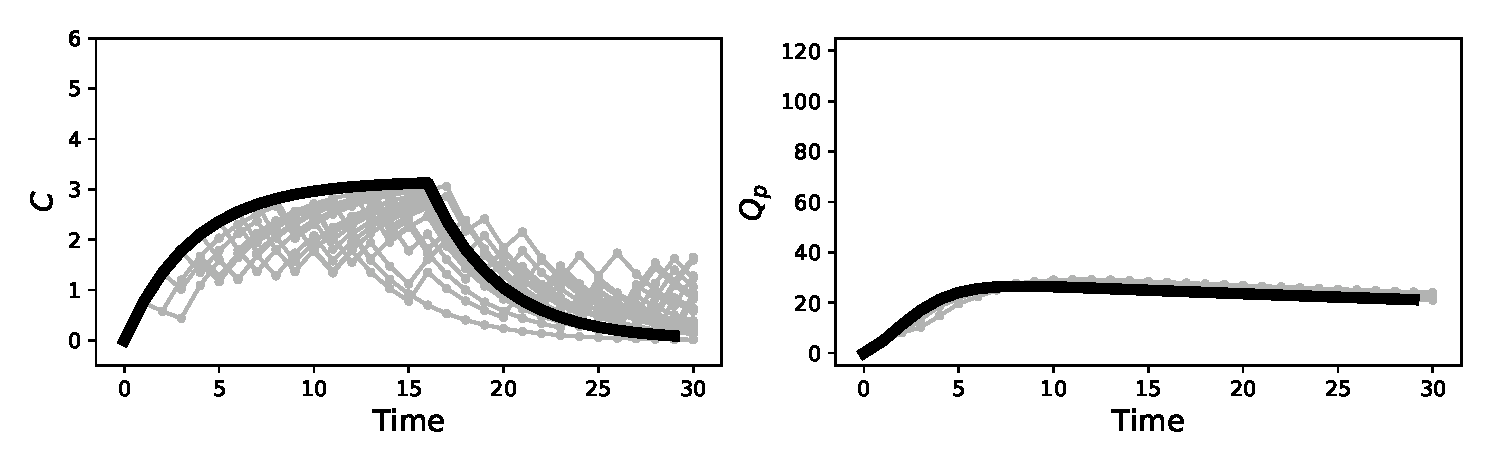
\includegraphics[width=0.4\textwidth]{cancer_no_influential_transitions_partial.eps}}
    \subfigure[Dead end sequence]{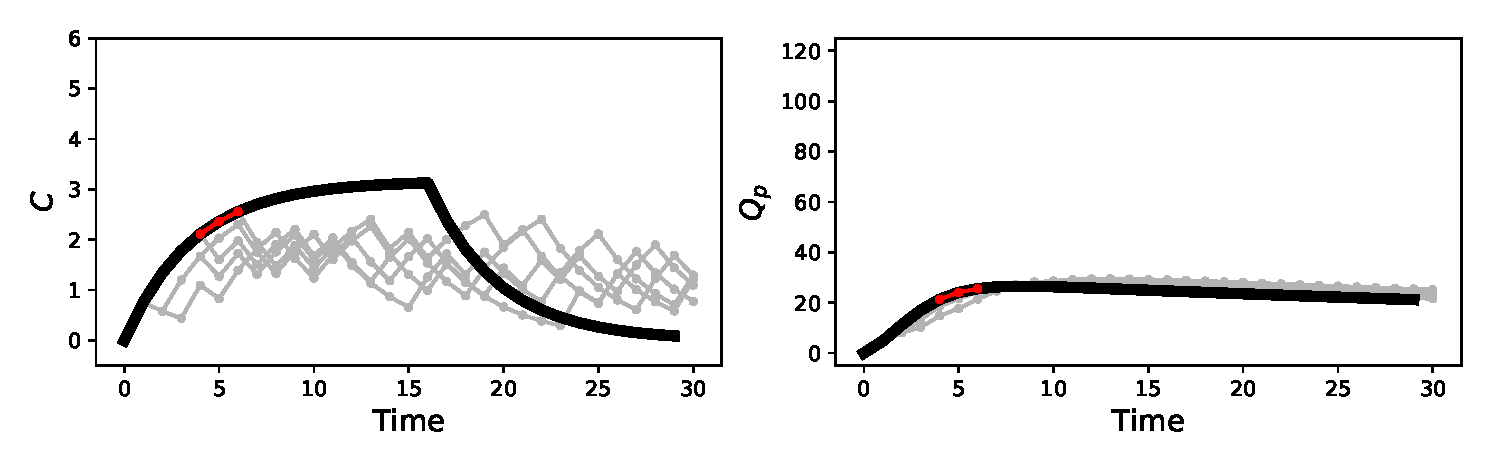
\includegraphics[width=0.4\textwidth]{cancer_dead_end_partial.eps}}
    \subfigure[Highlighted reliable transitions]{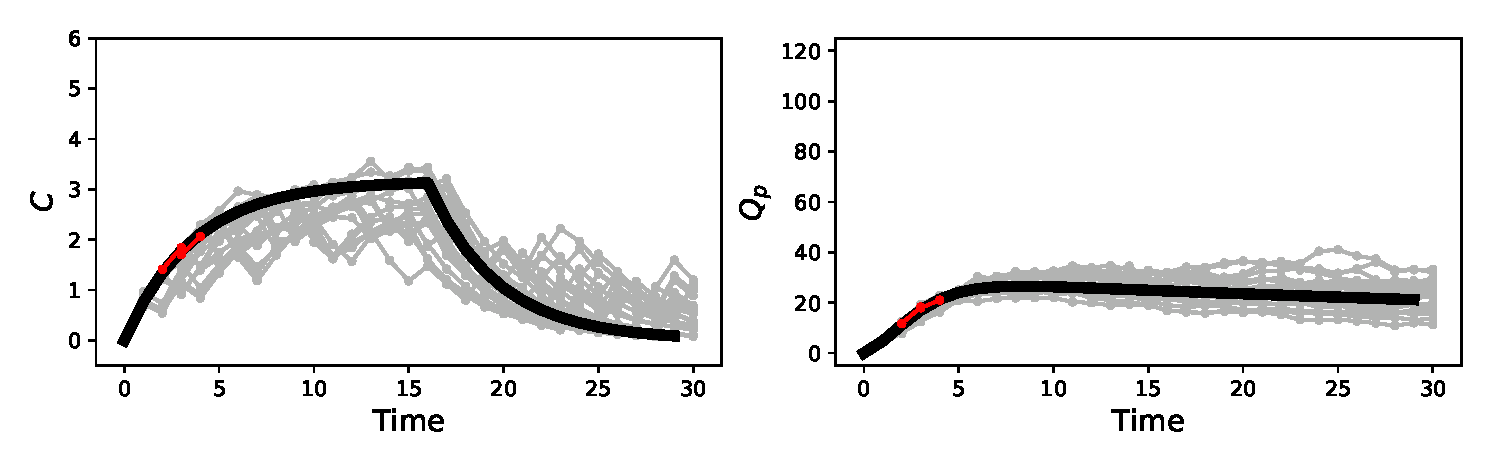
\includegraphics[width=0.4\textwidth]{cancer_influential_good_transitions_partial.eps}}
    \subfigure[Highlighted problematic transitions]{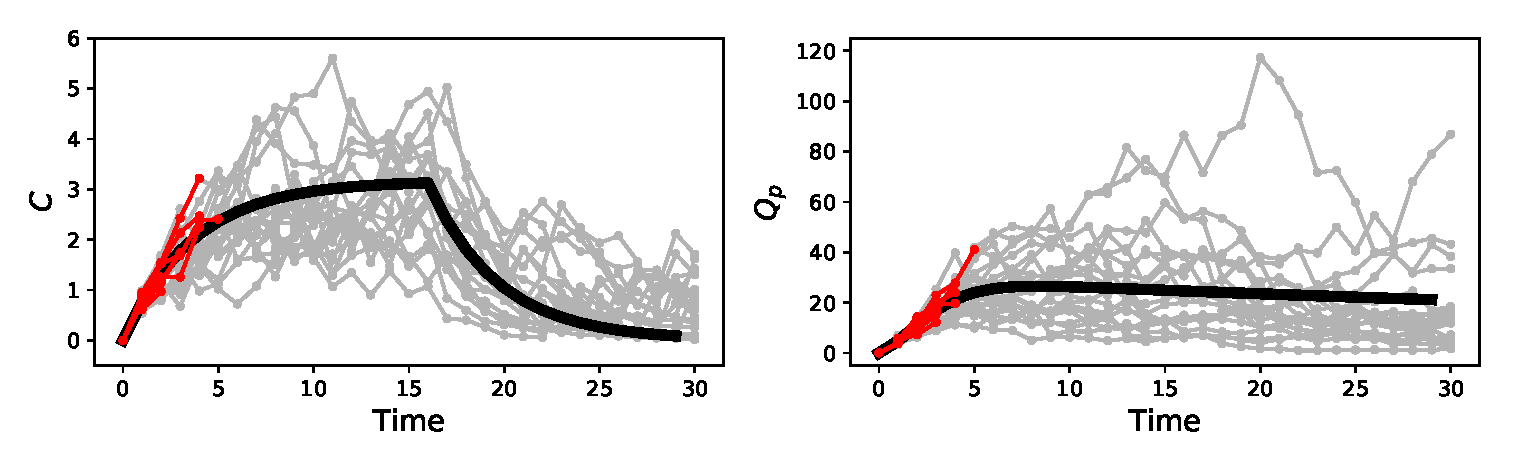
\includegraphics[width=0.4\textwidth]{cancer_recognizable_bad_transitions_partial.eps}}
    \caption{\textbf{Influence analysis for simulated cancer data.} Analysis of synthetic cancer simulations demonstrates how influence analysis can differentiate between different diagnostics of the OPE process.}
    \label{fig:cancer}
\end{figure}

To demonstrate the different ways in which influence analysis can allow domain experts to either increase our confidence in the validity of OPE or identify instances where they are invalid, we first present results on a simulator of cancer dynamics. The 4 dimensional states of the simulator approximate the dynamics of tumor growth, with actions consisting administration of chemotherapy at each timestep representing one month. For more details see \citet{ribba2012tumor}.

In Figure \ref{fig:cancer} we present four cases in which we attempt to evaluate the policy of treating a patient for 15 months and then discontinuing chemotherapy until the end of treatment at 30 months. Each subplot in Figure \ref{fig:cancer} shows two of the four state variables as a function of time, under different conditions which might make evaluation more difficult, such as difference in behavior policy or stochasticity in the environment. The heavy black line represents the expectation of each state dimension at each time-step under the evaluation policy, while the grey lines represent observed transitions under the behavior policy which is $\epsilon$-greedy with respect to the evaluation policy. In all figures, we highlight in red all influential transitions our method would have highlighted for review by domain experts $(\tilde{I}_c = 0.05)$.

\paragraph{Case 1: OPE seems reliable.}
Figure \ref{fig:cancer}(a) represents a typical example where the OPE can easily be trusted. Despite the large difference between the evaluation and behavior policy $(\epsilon = 0.3)$, enough trajectories have been observed in the data to allow for proper evaluation, and no transition is flagged as being too influential. The value estimation error in this example is less than $1\%$ and our method correctly labels this dataset as reliable.

\paragraph{Case 2: Unevaluatable.}
Figure \ref{fig:cancer}(b) is similar in experimental conditions to (a) ($\epsilon = 0.3$ and deterministic transitions), but with less collected data, so that the observations needed to properly estimate the dynamics are not in the data. This can be seen by the lack of overlap between the observed transitions and the expected trajectory, and results in a $38\%$ value estimation error. In real life we will not know what the expected trajectory under the evaluation policy looks like, and therefore will not be able to make the comparison and detect the lack of overlap between transitions under the evaluation and behavior policies. However, our method highlights a very influential sequence which terminates at a dead-end, and thus will correctly flag this dataset as not sufficient for evaluation. Our method in this case is confident enough to dismiss the results of evaluation without need for domain experts, but can still inform experts on what type of data is lacking in order for evaluation to be feasible.

\paragraph{Case 3: Humans might help.}
In Figures \ref{fig:cancer}(c-d), $\epsilon = 0.3$, but the dynamics have different levels of stochasticity. The less stochastic dynamics in \ref{fig:cancer}(c) allow for relatively accurate evaluation ($8\%$ error) but our method identifies several influential transitions which must be presented to a domain expert. These transitions lie on the expected trajectory, and thus a clinician would verify that they represent a typical response of a patient to treatment. This is an example in which our method would allow a domain expert to verify the validity of the evaluation by examining the flagged influential transitions.

Conversely, in \ref{fig:cancer}(d) some extreme outliers lead to a large estimation error ($23\%$ error). The influential transitions identified by our method are exactly those which start close to the expected trajectory but deviate significantly from the expected dynamics. A domain expert presented with the these transitions would easily be able to note that the OPE heavily relies on atypical patients and rightly dismiss the validity of evaluation.

To summarize this section, we demonstrated that analysis of influences can both validate or invalidate the evaluation without need for domain experts, and in intermediate cases present domain experts with the correct queries required to gain confidence in the evaluation results or dismiss them.

\subsection{Analysis of real ICU data - MIMIC III}

\begin{figure*}[t]
\centering
\includegraphics[width=0.43\textwidth]{ID-226662_trans-8.pdf}
\includegraphics[width=0.43\textwidth]{ID-233975_trans-10.pdf}
\caption{Influence analysis on our real-world dataset discovered six transitions in the evaluation dataset that were especially influential on our OPE. We display two of them in this figure, see Appendix \ref{sec:additional-mimic-results} for the remaining four.} 
\label{fig:mimic}
\end{figure*}

To show how influence analysis can help debug OPE for a challenging healthcare task, we consider the management of acutely hypotensive patients in the ICU. Hypotension is associated with high morbidity and mortality \citep{jones2006emergency}, but management of these patients is not standardized as ICU patients are heterogeneous. Within critical care, there is scant high-quality evidence from randomized controlled trials to inform treatment guidelines \citep{de2018unexplained,girbes2019time}, which provides an opportunity for RL to help learn better treatment strategies. In collaboration with an intensivist, we use influence analysis to identify potential artefacts when performing OPE on a clinical dataset of acutely hypotensive patients. 

\paragraph{Data and evaluation policy.}
Our data source is a subset of the publicly available MIMIC-III dataset \citep{johnson2016mimic}. See Appendix \ref{appendix:mimic_details} for full details of the data preprocessing. Our final dataset consists of 346 patient trajectories (6777 transitions) for learning a policy and another 346 trajectories (6863 transitions) for evaluation of the policy via OPE and influence analysis. 

Our state space consists of 29 relevant clinical variables, summarizing current physiological condition and past actions. The two main treatments for hypotension are administration of an intravenous (IV) fluid bolus or initiation of vasopressors. We bin doses of each treatment into 4 categories for "none", "low", "medium" and "high", so that the full action space consists of 16 discrete actions. Each reward is a function of the next blood pressure (MAP) and takes values in $[-1,0]$. As an evaluation policy, we use the most common action of a state's 50 nearest neighbors. This is setup is equivalent to constructing a decision assistance tool for clinicians by recommending the common practice action for patients, and using OPE combined with influence analysis to estimate the efficacy of such a tool. See Appendix \ref{appendix:mimic_details} for more details on how we setup the RL problem formulation, and for the kernel function used to compute nearest-neighbors. 

\paragraph{Presenting queries to a practicing intensivist.}
Running influence analysis flags 6 influential transitions that have high influence, which we define as a change of 5\% or more on the final value estimate. We show 2 of these transitions in Figure \ref{fig:mimic} and the rest in Appendix \ref{sec:additional-mimic-results}. While this analysis highlights individual transitions, our results figures display additional context before and after the suspect transition to help the clinician understand what might be going on.

In Figure \ref{fig:mimic}, each column shows a transition flagged by influence analysis. The top two rows show actions taken (actual treatments in the top row and binned actions in the second row). The remaining three rows show the most important state variables that inform the clinicians' decisions: blood pressure (MAP), urine output, and level of consciousness (GCS). For these three variables, the abnormal range is shaded in red, where the blood pressure shading is darker highlighting its direct relationship with the reward. Vertical grey lines represent timesteps, and the highlighted influential transition is shaded in grey.

\paragraph{Outcome: Identifying and removing an influential, buggy measurement.}
The two transitions in Figure \ref{fig:mimic} highlight potential problems in the dataset that have a large effect on our final OPE estimate. In the first transition (left), a large drop in blood pressure is observed at the starting time of this transition, potentially leaving the patient in a dangerous hypotensive state. Suprisingly, the patient received no treatment, and this unusual transition has a 29\% influence on the OPE estimate. Given additional context just before and after the transition, though, it was clear to the clinician that this was due to a single low measurement in a sequence that was previously stable. Coupled with a stable GCS (patient was conscious and alert) and a normal urine output, the intensivist easily determined the single low MAP was likely either a measurement error or a clinically insignificant transient episode of hypotension. After correcting the outlier MAP measurement to its most recent normal value (80mmHg) and then rerunning FQE and the influence analysis, the transition no longer has high influence and was not flagged.

\paragraph{Outcome: Identifying and correcting a temporal misalignment.}
The second highlighted transition (right) features a sudden drop in GCS and worsening MAP values, indicating a sudden deterioration of the patient's state, but treatment is not administered until the next timestep. The intensivist attributed this finding to a time stamp recording error. Again, influence analysis identified an inconsistency in the original data which had undue impact on evaluation. After correcting the inconsistency by shifting the two fluid treatments back by one timestep each, we found that the transition no longer had high influence and was not flagged.

\section{Discussion}

A key aim of this paper is to formulate a framework for using domain expertise to help in evaluating the trustworthiness of OPE methods for noisy and confounded observational data. The motivation for this research direction is the intersection of two realities: for messy real-world applications, the data itself might never be enough; and domain experts will always need to be involved in the integration of decision support tools in the wild, so we should incorporate their expertise into the evaluation process. We showcased influence analysis as one way of performing this task for value-based OPE, but emphasize that such measures can and should be incorporated into other OPE methods as well. For example, importance sampling weights offer a straightforward way of highlighting important entire trajectories for IS based techniques, and the dynamics learned by models in model-based OPE can be tested for their agreement with expert intuition.

We stress that research to integrate human input into OPE methods to increase their reliability complements, and does not replace, the approaches for estimating error bounds and uncertainties over the errors of OPE estimates. The fact that traditional theoretical error bounds rely so heavily on assumptions which are generally impossible to verify from the data alone highlights the need for other techniques for gauging to what extent these assumptions hold.

\bibliography{references}
\bibliographystyle{icml2020}

\end{document}


